\begin{figure}
\centering

% Left column: two stacked figures
\begin{minipage}{0.29\textwidth}
    \begin{subfigure}{\textwidth}
        \centering
        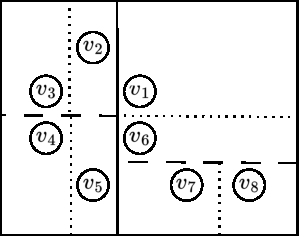
\includegraphics[width=\textwidth]{images/sfc_adaptive.svg.pdf}
        \caption{}
        \label{fig:sfc_adaptive}
    \end{subfigure}

    % \vspace{0.5cm} % Adjust spacing as needed

    \begin{subfigure}{\textwidth}
        \centering
        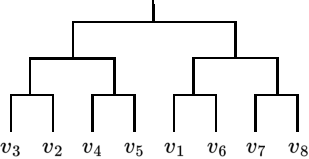
\includegraphics[width=\textwidth]{images/sfc_kdtree.svg.pdf}
        \caption{}
        \label{fig:sfc_kdtree}
    \end{subfigure}
\end{minipage}
\hfill
% Right column: one tall figure
\begin{minipage}{0.13\textwidth}
    \begin{subfigure}[b]{\textwidth}
        \centering
        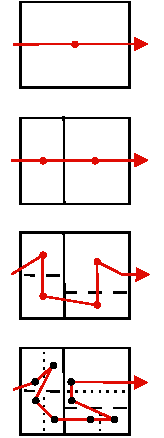
\includegraphics[width=\textwidth]{images/sfc_traversal.svg.pdf}
        \caption{}
        \label{fig:sfc_traversal}
    \end{subfigure}
\end{minipage}

\caption{The adaptive space-filling curve (SFC) partitioning process begins with the recursive spatial subdivision of the input domain (a), followed by the construction of the corresponding KD-tree (b). Then, a direction-aware recursive traversal defines a linear ordering of the leaf nodes (c). In this example, the resulting order is $v_3 \rightarrow v_2 \rightarrow v_4 \rightarrow v_5 \rightarrow v_7 \rightarrow v_8 \rightarrow v_6 \rightarrow v_1$.}
\label{fig:sfc}
\end{figure}